% This LaTeX was auto-generated from MATLAB code.
% To make changes, update the MATLAB code and export to LaTeX again.

\documentclass{article}

\usepackage[utf8]{inputenc}
\usepackage[T1]{fontenc}
\usepackage{lmodern}
\usepackage{graphicx}
\usepackage{color}
\usepackage{listings}
\usepackage{hyperref}
\usepackage{amsmath}
\usepackage{amsfonts}
\usepackage{epstopdf}
\usepackage[table]{xcolor}
\usepackage{matlab}

\sloppy
\epstopdfsetup{outdir=./}
\graphicspath{ {./Task5_images/} }

\begin{document}

\matlabtitle{实验五 网络优化}


\matlabheading{习题}

\matlabheadingtwo{1. 某公司在六个城市$C_1 ,C_2 ,C_3 ,C_4 ,C_5 ,C_6$中都有分公司,从$C_i$到$C_j$的直达航班票价有下述矩阵的第$i$行、第$j$列元素给出($\infty$表示无直达航班),该公司想算出一张任意两个城市之间最廉价线路表,试作出这样的表来。}

\begin{par}
$$\left\lbrack \begin{array}{cccccc}
0 & 50 & \infty  & 40 & 25 & 10\\
50 & 0 & 15 & 20 & \infty  & 25\\
\infty  & 15 & 0 & 10 & 20 & \infty \\
40 & 20 & 10 & 0 & 10 & 25\\
25 & \infty  & 20 & 10 & 0 & 55\\
10 & 25 & \infty  & 25 & 55 & 0
\end{array}\right\rbrack$$
\end{par}

\begin{matlabcode}
A = [
    0 50 0 40 25 10;
    50 0 15 20 0 25;
    0 15 0 10 20 0;
    40 20 10 0 10 25;
    25 0 20 10 0 55;
    10 25 0 25 55 0;
    ];
G = digraph(A);
list = string(nan(6));
for i = 1 : 6
    for j = 1 : 6
        list(i, j) = string(mat2str(shortestpath(G, i, j)));
    end
end
list
\end{matlabcode}
\begin{matlabtableoutput}
list = 
    "1"          "[1 6 2]"    "[1 5 4 3]"    "[1 5 4]"    "[1 5]"      "[1 6]"  
    "[2 6 1]"    "2"          "[2 3]"        "[2 4]"      "[2 4 5]"    "[2 6]"  
    "[3 5 1]"    "[3 2]"      "3"            "[3 4]"      "[3 5]"      "[3 4 6]"
    "[4 5 1]"    "[4 2]"      "[4 3]"        "4"          "[4 5]"      "[4 6]"  
    "[5 1]"      "[5 4 2]"    "[5 4 3]"      "[5 4]"      "5"          "[5 1 6]"
    "[6 1]"      "[6 2]"      "[6 4 3]"      "[6 4]"      "[6 1 5]"    "6"      

\end{matlabtableoutput}


\matlabheadingtwo{2. 求下图中每一结点到其他结点的最短路。}

\begin{matlabcode}
A = [
    0 3 10 0 0 0 0 0;
    3 0 0 5 0 0 0 0;
    10 0 0 6 0 0 0 0;
    0 5 6 0 4 0 10 0;
    0 0 0 4 0 9 5 0;
    0 0 0 0 9 0 3 4;
    0 0 0 10 5 3 0 6;
    0 0 0 0 0 4 6 0;
];
G = graph(A, ["v_1", "v_2", "v_3", "v_4", "v_5", "v_6", "v_7", "v_8"]);
plot(G, "EdgeLabel", G.Edges.Weight, "XData", [0 0 1 1 2 3 2 3], "YData", [1 0 1 0 1 1 0 0]);
xlim([-0.5, 3.5]);
ylim([-1, 2]);
\end{matlabcode}
\begin{center}
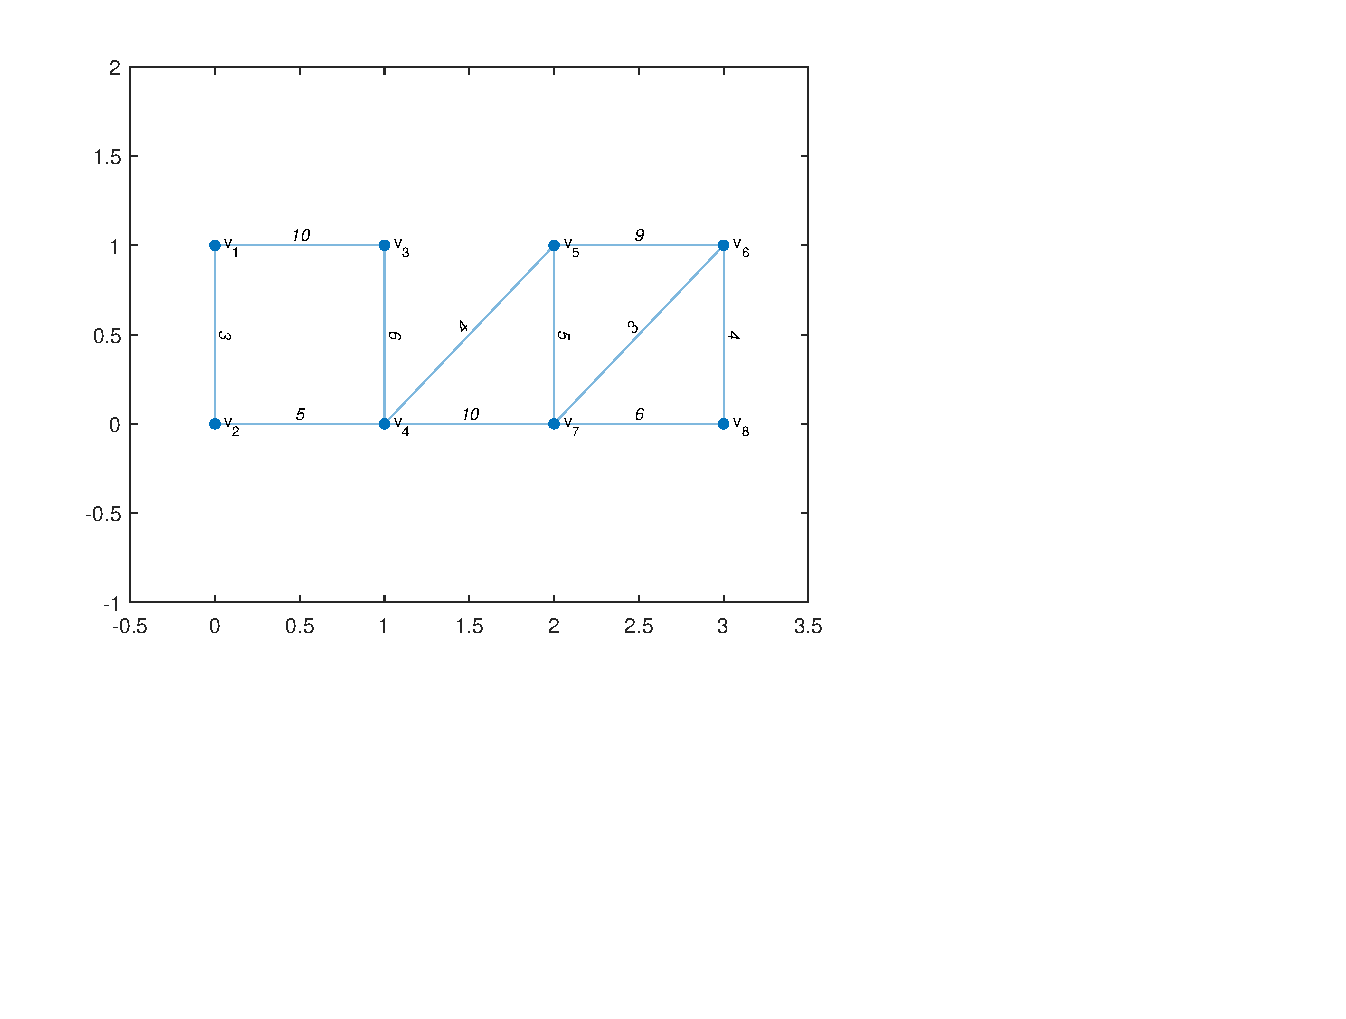
\includegraphics[width=\maxwidth{56.196688409433015em}]{figure_0}
\end{center}
\begin{matlabcode}
distances(G)
\end{matlabcode}
\begin{matlaboutput}
ans = 8x8    
     0     3    10     8    12    20    17    23
     3     0    11     5     9    17    14    20
    10    11     0     6    10    18    15    21
     8     5     6     0     4    12     9    15
    12     9    10     4     0     8     5    11
    20    17    18    12     8     0     3     4
    17    14    15     9     5     3     0     6
    23    20    21    15    11     4     6     0

\end{matlaboutput}


\matlabheadingtwo{3. 在一个城市交通系统中取出一段,其入口为顶点$v_1$,出口为顶点$v_8$,每条弧段旁的数字表示通过该路段所需时间,每次转弯所需要附加时间为�$3$,求$v_1$到$v_8$的最短时间路径。}

\begin{matlabcode}
A = [
    0 1 0 0 0 0 0 0;
    1 0 3 2 0 0 0 0;
    0 3 0 0 1 0 0 0;
    0 2 0 0 0 0 2 0;
    0 0 1 0 0 6 2 0;
    0 0 0 0 6 0 0 3;
    0 0 0 2 2 0 0 4;
    0 0 0 0 0 3 4 0;
];
G = graph(A, ["v_1" "v_2" "v_3" "v_4" "v_5" "v_6" "v_7" "v_8"]);
plot(G, "XData", [0 1 2 1 3 4 3 4], "YData", [1 1 1 0 1 1 0 0], "EdgeLabel", G.Edges.Weight);
xlim([-0.5, 4.5]);
ylim([-1.5, 2.5]);
\end{matlabcode}
\begin{center}
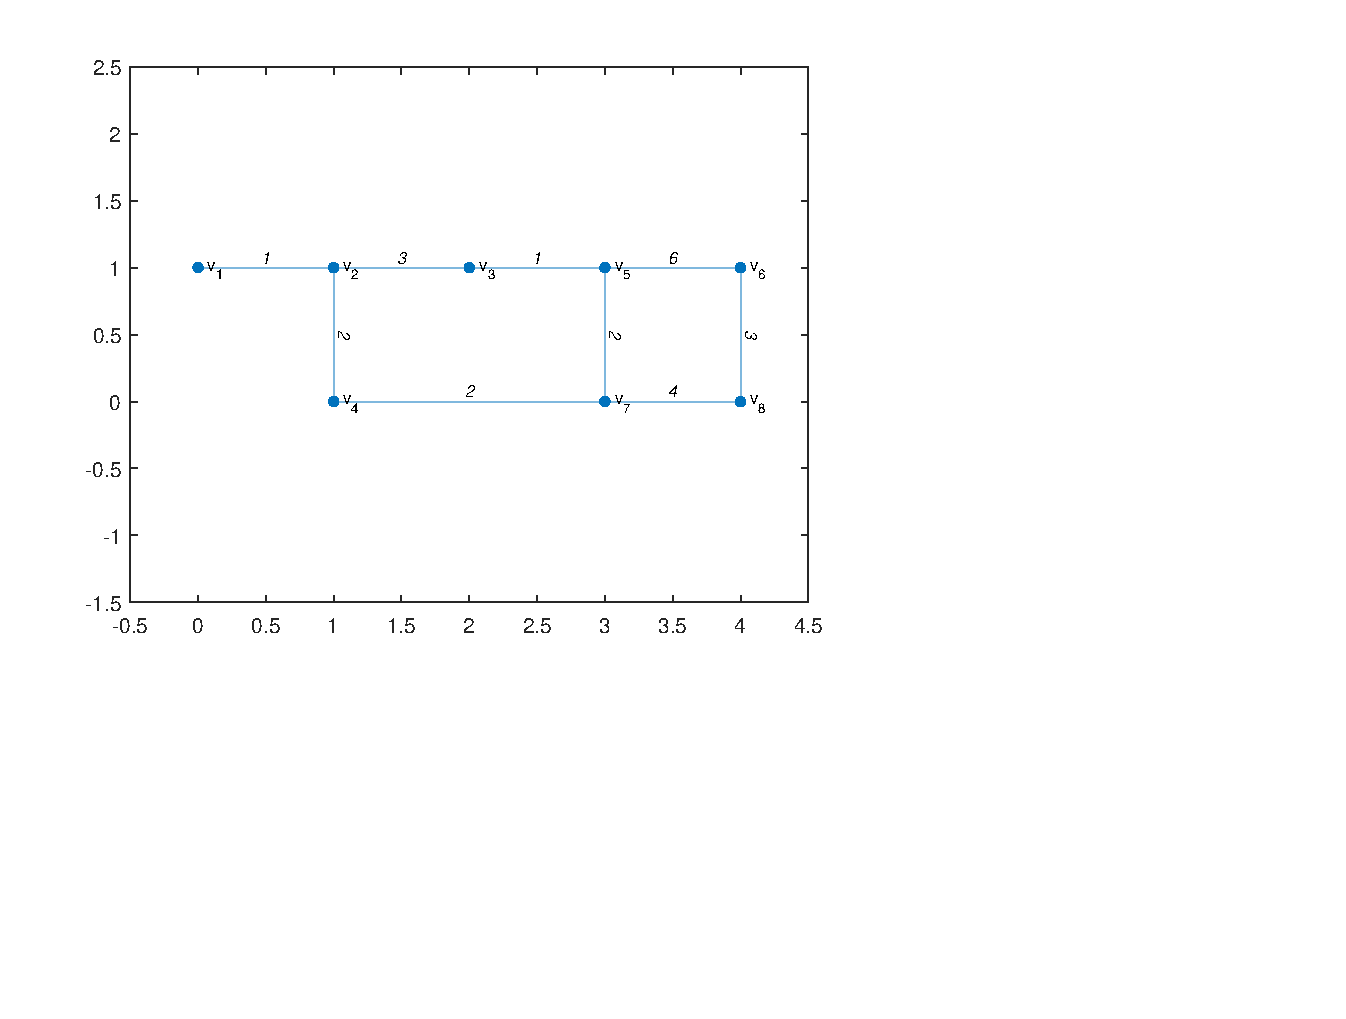
\includegraphics[width=\maxwidth{56.196688409433015em}]{figure_1}
\end{center}
\begin{matlabcode}
% 由于个别结点存在转弯时间,将转弯时间归入路径时间,得到新的图
A = [
    0 1 0 0 0 0 0 0;
    1 0 3 5 0 0 0 0;
    0 3 0 0 1 0 0 0;
    0 5 0 0 0 0 5 0;
    0 0 1 0 0 6 8 0;
    0 0 0 0 6 0 0 6;
    0 0 0 5 8 0 0 4;
    0 0 0 0 0 6 4 0;
];
G = graph(A, ["v_1" "v_2" "v_3" "v_4" "v_5" "v_6" "v_7" "v_8"]);
plot(G, "XData", [0 1 2 1 3 4 3 4], "YData", [1 1 1 0 1 1 0 0], "EdgeLabel", G.Edges.Weight);
xlim([-0.5, 4.5]);
ylim([-1.5, 2.5]);
\end{matlabcode}
\begin{center}
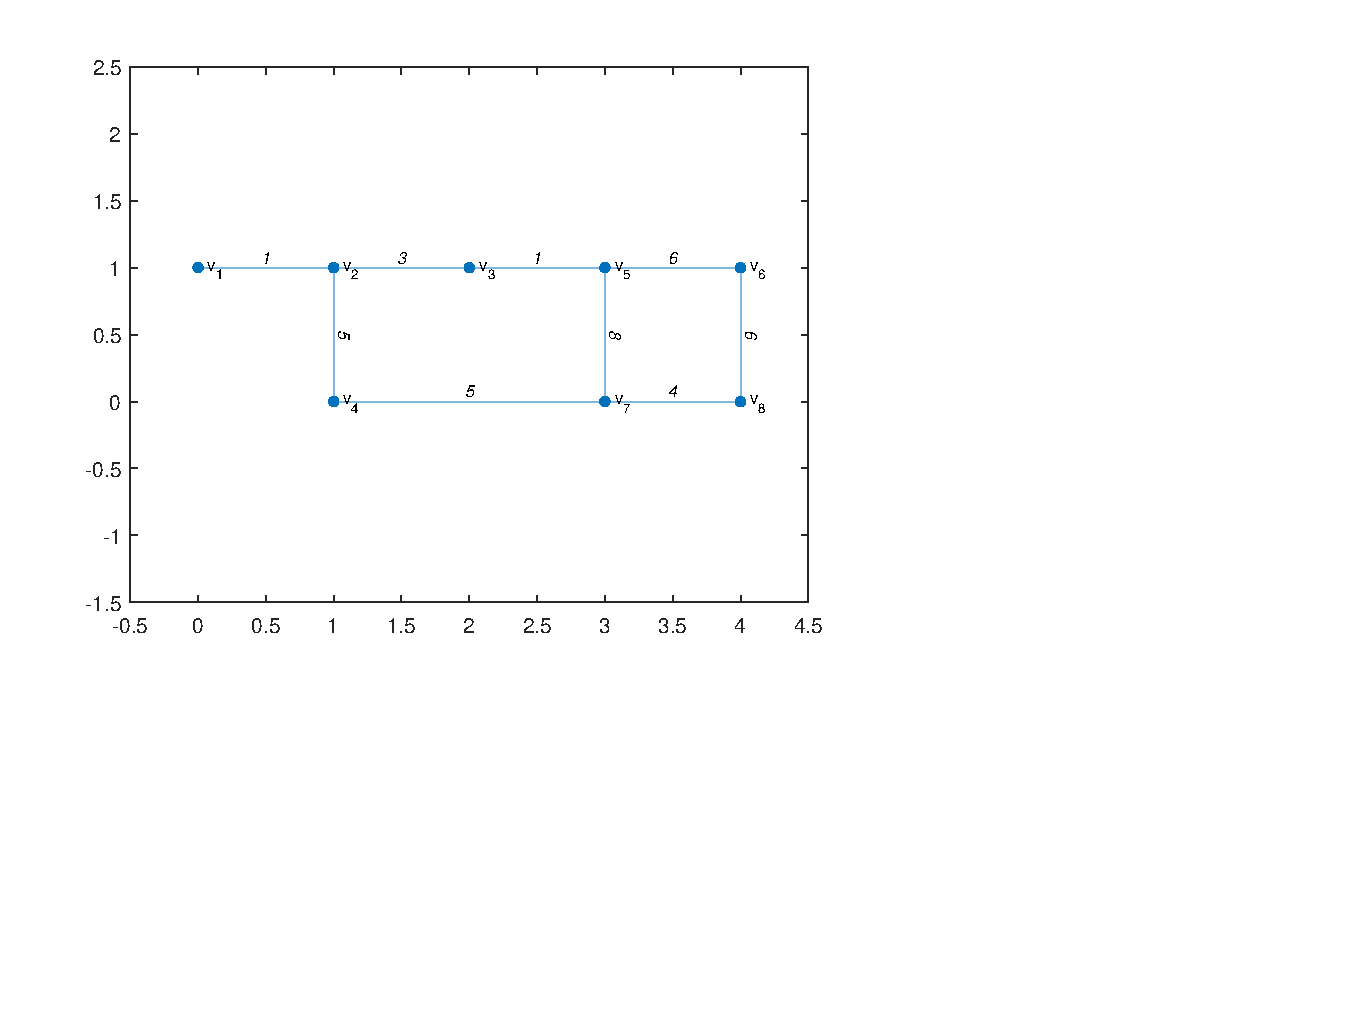
\includegraphics[width=\maxwidth{56.196688409433015em}]{figure_2}
\end{center}
\begin{matlabcode}
[route, dist] = shortestpath(G, "v_1", "v_8")
\end{matlabcode}
\begin{matlabtableoutput}
route = 
    "v_1"    "v_2"    "v_4"    "v_7"    "v_8"

\end{matlabtableoutput}
\begin{matlaboutput}
dist = 15
\end{matlaboutput}

\end{document}
